% Kapitel 1 Arbeitsgrundlagen------------------------------------------------- %
\section{Arbeitsgrundlagen}
% ---------------------------------------------------------------------------- %
In diesem Abschnitt werden die Arbeitsgrundlagen zur Beugung und Interferenz für den Versuch erarbeitet.
% **************************************************************************** %
\subsection{Huygenssches Prinzip}
% **************************************************************************** %
Das huygensche Prinzip besagt, dass jeder Punkt einer Wellenfläche als Ausgangspunkt einer Elementarwelle betrachtet werden kann, die sich mit gleicher Phasengeschwindigkeit und Wellenlänge wie die ursprüngliche Welle ausbreitet. Durch die Überlagerung sämtlicher Elementarwellen ergibt sich die neue Lage der Wellenfront. Es bildet sich eine rücklaufende Welle, da die Elementarwelle eine Kugelform hat.

\begin{figure}[h!]
	\centering
	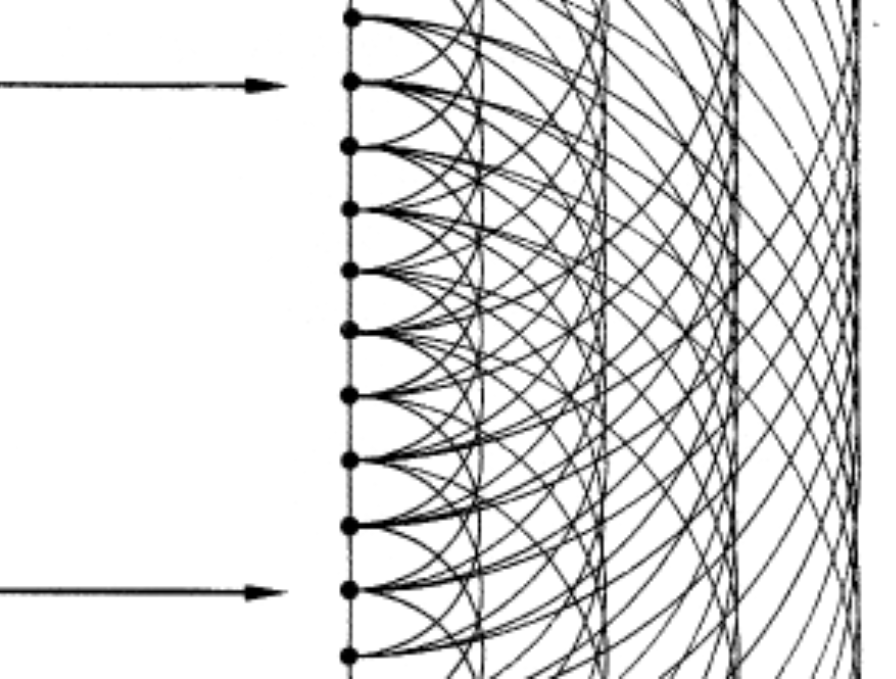
\includegraphics[width=0.8\textwidth]{data/huygens}
	\caption{Eine Welle die sich aus Überlagerungen von Kugelwellen bildet. Mit den schwarzen Punkten sind die Punkte, welcher von einer Wellenfront erreicht wird, dargestellt. Dies ist der Ausgangspunkt für eine kugelförmige Elementarwelle. }
	\label{fig:heygens}
\end{figure}

\newpage
\begin{figure}[h!]
	\centering
	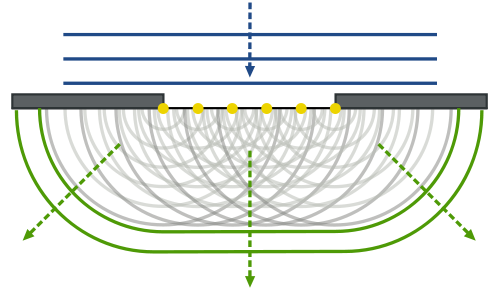
\includegraphics[width=0.5\textwidth]{data/hspalt.png}
	\caption{Beugung einer ebenen Wellenfront an einem Spalt nach dem huygensschen Prinzip.}
	\label{fig:heygens_spalt}
\end{figure}

In Abbildung \ref{fig:heygens_spalt} wird das huygensche Prinzip auf die Beugung von Licht an Hindernissen angewandt. Eine ebene Wellenfront wird an einem Spalt gebeugt. Es entsteht näherungsweise eine Rechtecksform. Nach dem Prinzip der Interferenz kann die resultierende Welle durch Superposition aller Elementarwellen berechnen lässt. 


%https://de.wikipedia.org/wiki/Huygenssches_Prinzip

%http://www.dieter-heidorn.de/Physik/SS/K03_Wellen/K03_Huygens/K03_Huygens.html


% **************************************************************************** %
\subsection{Beugungsintegral}
% **************************************************************************** %
Die Beugung von Licht an eine beliebig geformte Blende kann mit dem Beugungsintegral berechnet werden. Dieses Beugungsintegral basiert auf dem Modell der Elementarwellen. Für das Beugungsintegral gibt es zwei Näherungen. Für das Nahfeld wird die Fresnel-Näherung und für das Fernfeld die Fraunhofer-Näherung angewandt. Das System, welches mit mittels Kirchhoffischen Beugungsintegral beschrieben wird skizziert. Die Formel \ref{eq:integral} beschreibt wie man die Amplitude $ \phi_{P} $ im Punkt P auf dem Beobachtungsschirm berechnet werden kann. Die Berechnung ist Abhängig von der Amplitude der Quelle $ a_{Q} $, dem Betrag des Wellenvektors in der Quelle $ k_{0} = 2 \pi/\lambda $, der Wellenlänge $ \lambda $, den Neigungsfaktoren $ \theta $ und $ \theta_{1} $, den Abständen $ L $, $ L_{1} $, $ d $, $ d_{1} $ und der Blendfunktion $ f(s) $. Bei einer vollkommenen undurchlässigen Blende beträgt die Blendfunktion $ f(s)=0 $ und bei einer vollkommen durchlässigen Blende beträgt $ f(s)=1 $.

\begin{equation}\label{eq:integral}
\psi_{p}=\frac{a_{Q}\cdot k_{0}}{2\cdot \pi \cdot i} \cdot \iint_{Blende} f(s) \cdot\frac{e^{i\cdot k_{0}\cdot (d +d_{i})}}{d\cdot d_{1}} \cdot \left[ \frac{cos\theta + cos\theta_{1}}{2} \right] ds
\end{equation}

\begin{figure}[h!]
	\centering
	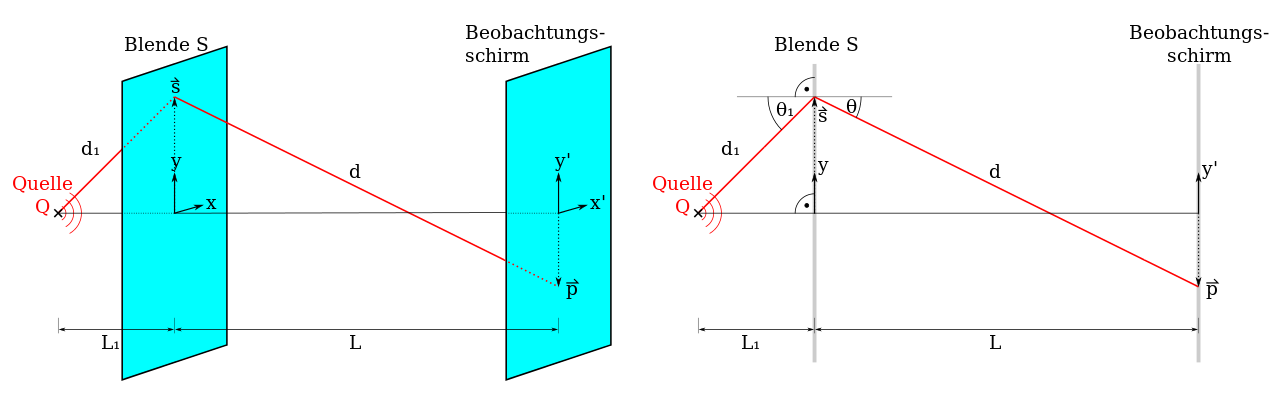
\includegraphics[width=0.7\textwidth]{data/skizze_beugungsintegral.png}
	\caption{Die Anordnung besteht aus einer Lichtquelle $ Q $, einer Blende $ S $, an der das Licht gebeugt wird und einem Beobachtungsschirm auf dem die auftreffende Lichtintensität an P untersucht wird.}
	\label{fig:integral}
\end{figure}

\newpage
% **************************************************************************** %
\subsection{Frauenhofer-Näherung}
% **************************************************************************** %
Die Fernfeld-Näherung des Beugungsintegral (Formel \ref{eq:integral}) entspricht die Frauenhofer-Näherung. Bei dieser Näherung wird angenommen, dass $ L\gg \arrowvert \overrightarrow{s} \arrowvert = \sqrt{x^2 + y^2} $ und $ L_{1} \gg \arrowvert \overrightarrow{p} \arrowvert = \sqrt{x_{p}^2 + y_{p}^2} $. Der Term mit den Neigungsfaktoren $ \theta $ und $ \theta_{1} $ kann in diesem Fall vernachlässigt werden. Zudem lässt sich wegen dieser Näherung $ d\cdot d_{1} $ im Nenner durch $ L\cdot L_{1} $ ersetzt. Der Ausdruck $ d + d_{1} $ im Exponent enthält die Information zur Phase, deshalb darf hier nicht $ d $ durch $ L $ ersetzt werden. Sie können jedoch mit einer Taylor-Reihe  vereinfacht werden. Wenn man diese Vereinfachungen vornimmt ergiebig sich die sogenannte Frauenhofer-Näherung, welche in der Formel \ref{eq:näherung} dargestellt ist. Sie lässt sich zur Formel \ref{eq:fourie} umformen, wenn man den Wellenvektor $ \overrightarrow{K} = \frac{k_{0}}{L} \cdot \overrightarrow{p}$ einführt. Somit ist der Term unter dem Doppelintegral über die Blende gerade die Fourier-Transformierte der Blendfunktion $ f(s) $.

\begin{equation}\label{eq:näherung}
\psi_{p}\approx \frac{a_{Q}\cdot k_{0}}{2\cdot \pi \cdot i} \cdot \frac{e^{i\cdot k_{0}\cdot (L1 +L+\frac{p^{2}}{2L})}}{L\cdot L_{1}} \cdot \iint_{Blende} f(s) \cdot e^{-i\cdot k_{0}\cdot \frac{((x\cdot x_{p} + y\cdot y_{p} ))}{L} } \cdot ds
\end{equation}

\begin{equation}\label{eq:fourie}
\psi_{p}\approx \frac{a_{Q}\cdot k_{0}}{2\cdot \pi \cdot i} \cdot \frac{e^{i\cdot k_{0}\cdot (L1 +L+\frac{p^{2}}{2L})}}{L\cdot L_{1}} \cdot \iint_{Blende} f(s) \cdot e^{-i\cdot \overrightarrow{K} \cdot \overrightarrow{s} } \cdot ds
\end{equation}

\newpage
\subsection{Frauenhofer'sche Beobachtungsart}
Bei der Frauenhofer'sche Beobachtungsart wird das Interfernzmuster, wie in der Abbildung \ref{fig:beobachtungsart} dargestellt, in der Brennebene beobachtet. Dies geschieht in dem das Interferenzmuster durch eine Linse auf einen Schirm projiziert wird. Die Linse wird im Abstand $ f $ vor dem Schirm platziert. Das beobachtete Muster ist bis auf einen Skalierungsfaktor identisch zum Interferenzmuster, welches in grosser Entfernung von den Quellen beobachtet werden kann. Der Abstand von der Linse von den Quellen hat keinen Einfluss auf die Abmessung oder die Form des Interferenzmuster. Er bestimmt nur den erfassten Winkelbereich.

\begin{figure}[h!]
	\centering
	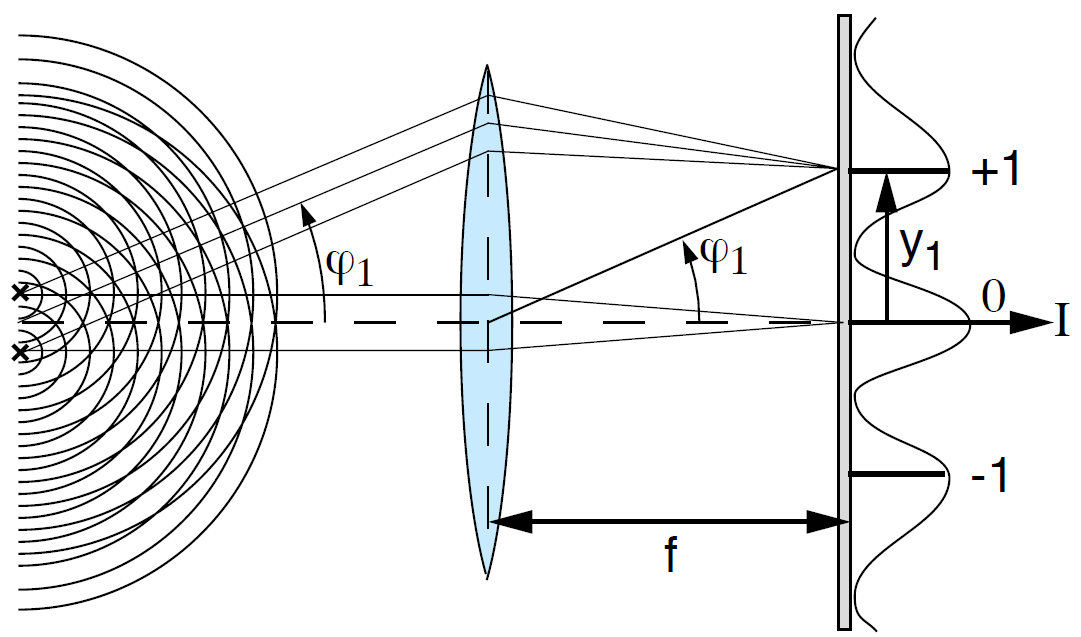
\includegraphics[width=0.8\textwidth]{data/fraunhofer}
	\caption{Frauenhofer'sche Beobachtungsart}
	\label{fig:beobachtungsart}
\end{figure}

Der Winkel $ \phi_{1} $ der Interferenz erster Ordnung kann mit dem Abstand $ y_{1} $ von dem Hauptstrahl zum Extrema der ersten Ordnung und der Brennweite $ f $ der Linse wie folgt berechnen.
\begin{equation}\label{eq:frauenhofer}
tan(\phi_{1}) =  \frac{y_{1}}{f}
\end{equation}
